\documentclass{beamer} % 使用 beamer 文档类
\usepackage{ctex, hyperref} % 中文支持和超链接
\usepackage[T1]{fontenc} % 字体编码
\newcommand{\myinstitution}{在此处输入您的机构名称 (Your Institution Name)} % 机构名称命令
\newcommand{\advisorname}{Your Advisor's Name} % 指导老师姓名命令
% 其他常用宏包
\usepackage{latexsym,amsmath,xcolor,multicol,booktabs,calligra}
\usepackage{graphicx,pstricks,listings,stackengine}

% 作者、标题等信息设置
\author[PresenterName]{Your Name \texorpdfstring{\newline Advisor: \advisorname}{, Advisor: \advisorname}} % [短版本]用于footline,{长版本}用于titlepage
\title{在此处输入您的演示文稿标题 (Your Presentation Title Here)} % 演示文稿标题
\subtitle{在此处输入副标题 (Your Subtitle Here) (可选)} % 副标题(可选)
\institute{\myinstitution} % 机构名称
\date{\today} % 日期
\usepackage{JOU} % 导入自定义 JOU 主题,可根据需要修改 JOU.sty 或替换为其他主题

% 自定义命令和颜色
\def\cmd#1{\texttt{\color{red}\footnotesize $\backslash$#1}} % 显示命令
\def\env#1{\texttt{\color{blue}\footnotesize #1}} % 显示环境
\definecolor{deepblue}{rgb}{0,0,0.5} % 深蓝色
\definecolor{deepred}{rgb}{0.6,0,0} % 深红色
\definecolor{deepgreen}{rgb}{0,0.5,0} % 深绿色
\definecolor{halfgray}{gray}{0.55} % 灰色

% 代码高亮设置
\lstset{
    basicstyle=\ttfamily\small,
    keywordstyle=\bfseries\color{deepblue},
    emphstyle=\ttfamily\color{deepred},    % 自定义高亮风格
    stringstyle=\color{deepgreen},
    numbers=left,
    numberstyle=\small\color{halfgray},
    rulesepcolor=\color{red!20!green!20!blue!20},
    frame=shadowbox,
}

\begin{document}

\kaishu % 设置楷体(中文)
\begin{frame}
    \titlepage % 标题页
    \begin{figure}[htpb]
        \centering
        \vspace{-6mm}
        
\includegraphics[width=0.18\linewidth]{pic/JOU_logo.jpg} % 插入校徽
    \end{figure}
\end{frame}

\begin{frame}
\tableofcontents[sectionstyle=show,subsectionstyle=show/shaded/hide,subsubsectionstyle=show/shaded/hide] % 目录
\end{frame}

%------------------- 课题背景 -------------------
\section{课题背景}

\begin{frame}{用Beamer制作演示文稿的优势}
    \begin{itemize}[<+-| alert@+>]
        \item \LaTeX{} 是学术界广泛使用的排版系统,许多高校提供基于 \LaTeX{} Beamer 的演示文稿模板。
        \item 使用 Xe\LaTeX{} 编译选项可获得良好的中文支持。
        \item 本模板的 GitHub 项目地址位于 \url{https://github.com/TsekaLuk/JOU-Presentation-Beamer-Template}。如有模板相关的疑问或建议,可在此处提出。
    \end{itemize}
\end{frame}

%------------------- 研究现状 -------------------
\section{研究现状}

\subsection{Beamer主题参考}

\begin{frame}
    \begin{itemize}
        \item \LaTeX{} 系统自带多种基础 Beamer 主题。
        \item 国内外许多高校亦有其定制的 Beamer 主题,例如清华大学等。
        \item 本 JOU Beamer 主题的原始参考来源为:\newline \url{https://www.latexstudio.net/archives/4051.html}
    \end{itemize}
\end{frame}

%------------------- 研究内容 -------------------
\section{研究内容}

\subsection{本JOU Beamer主题特点}

\subsection{如何更好地做Beamer}

\begin{frame}{Why Beamer}
    \begin{itemize}
        \item \LaTeX 广泛用于学术界,期刊会议论文模板
    \end{itemize}
    \begin{table}[h]
        \centering
        \begin{tabular}{c|c}
            Microsoft\textsuperscript{\textregistered}  Word & \LaTeX \\
            \hline
            文字处理工具 & 专业排版软件 \\
            容易上手,简单直观 & 容易上手 \\
            所见即所得 & 所见即所想,所想即所得 \\
            高级功能不易掌握 & 进阶难,但一般用不到 \\
            处理长文档需要丰富经验 & 和短文档处理基本无异 \\
            花费大量时间调格式 & 无需担心格式,专心作者内容 \\
            公式排版差强人意 & 尤其擅长公式排版 \\
            二进制格式,兼容性差 & 文本文件,易读、稳定 \\
            付费商业许可 & 自由免费使用 \\
        \end{tabular}
    \end{table}
\end{frame}

\begin{frame}{排版举例}
    \begin{exampleblock}{无编号公式} % 使用 * 号去除编号
        \begin{equation*}
            J(\theta) = \mathbb{E}_{\pi_\theta}[G_t] = \sum_{s\in\mathcal{S}} d^\pi (s)V^\pi(s)=\sum_{s\in\mathcal{S}} d^\pi(s)\sum_{a\in\mathcal{A}}\pi_\theta(a|s)Q^\pi(s,a)
        \end{equation*}
    \end{exampleblock}
    \begin{exampleblock}{多行多列公式\footnote{如果公式中有文字出现,请用 $\backslash$mathrm\{\} 或者 $\backslash$text\{\} 包含,不然就会变成 $clip$,在公式里看起来比 $\mathrm{clip}$ 丑非常多。}}
        % 使用 & 分隔对齐
        \begin{align}
            Q_\mathrm{target}&=r+\gamma Q^\pi(s^\prime, \pi_\theta(s^\prime)+\epsilon)\\
            \epsilon&\sim\mathrm{clip}(\mathcal{N}(0, \sigma), -c, c)\nonumber
        \end{align}
    \end{exampleblock}
\end{frame}

\begin{frame}
    \begin{exampleblock}{编号多行公式}
        % 取自 Mathmode.tex
        \begin{multline}
            A=\lim_{n\rightarrow\infty}\Delta x\left(a^{2}+\left(a^{2}+2a\Delta x+\left(\Delta x\right)^{2}\right)\right.\label{eq:reset}\\
            +\left(a^{2}+2\cdot2a\Delta x+2^{2}\left(\Delta x\right)^{2}\right)\\
            +\left(a^{2}+2\cdot3a\Delta x+3^{2}\left(\Delta x\right)^{2}\right)\\
            +\ldots\\
            \left.+\left(a^{2}+2\cdot(n-1)a\Delta x+(n-1)^{2}\left(\Delta x\right)^{2}\right)\right)\\
            =\frac{1}{3}\left(b^{3}-a^{3}\right)
        \end{multline}
    \end{exampleblock}
\end{frame}

\begin{frame}{图形与分栏}
    % 以下为分栏与图形示例,左侧为pstricks绘图,右侧为图片
    \begin{minipage}[c]{0.3\linewidth}
        \psset{unit=0.8cm}
        \begin{pspicture}(-1.75,-3)(3.25,4)
            \psline[linewidth=0.25pt](0,0)(0,4)
            \rput[tl]{0}(0.2,2){$\vec e_z$}
            \rput[tr]{0}(-0.9,1.4){$\vec e$}
            \rput[tl]{0}(2.8,-1.1){$\vec C_{ptm{ext}}$}
            \rput[br]{0}(-0.3,2.1){$\theta$}
            \rput{25}(0,0){%
            \psframe[fillstyle=solid,fillcolor=lightgray,linewidth=.8pt](-0.1,-3.2)(0.1,0)}
            \rput{25}(0,0){%
            \psellipse[fillstyle=solid,fillcolor=yellow,linewidth=3pt](0,0)(1.5,0.5)}
            \rput{25}(0,0){%
            \psframe[fillstyle=solid,fillcolor=lightgray,linewidth=.8pt](-0.1,0)(0.1,3.2)}
            \rput{25}(0,0){\psline[linecolor=red,linewidth=1.5pt]{->}(0,0)(0.,2)}
            \psline[linecolor=red,linewidth=1.25pt]{->}(0,0)(0,2)
            \psline[linecolor=red,linewidth=1.25pt]{->}(0,0)(3,-1)
            \psline[linecolor=red,linewidth=1.25pt]{->}(0,0)(2.85,-0.95)
            \psarc{->}{2.1}{90}{112.5}
            \rput[bl](.1,.01){C}
        \end{pspicture}
    \end{minipage}\hspace{1cm}
    \begin{minipage}{0.5\linewidth}
        \medskip
        % 右侧插入图片
        \begin{figure}[h]
            \centering
            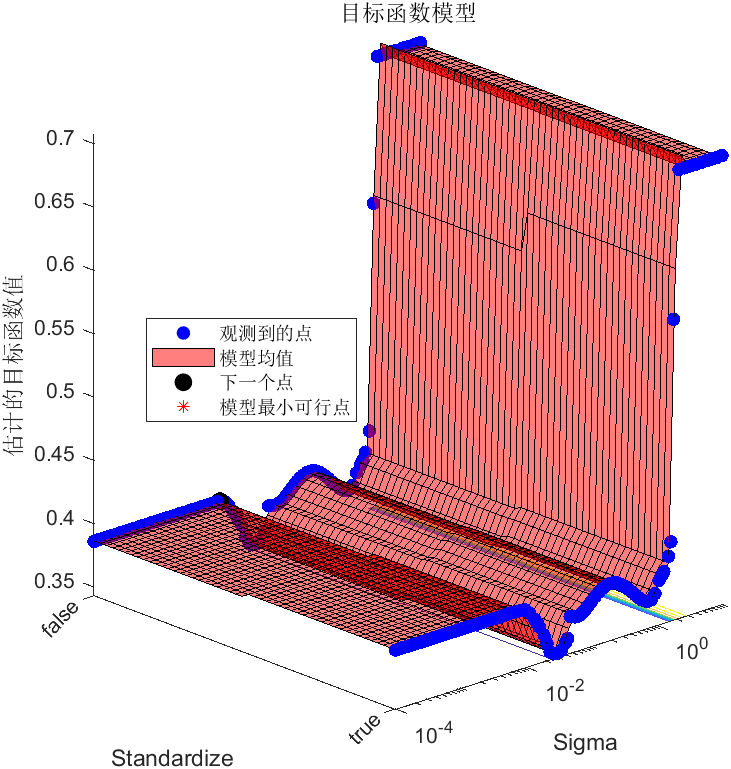
\includegraphics[height=.7\textheight]{pic/高斯回归+贝叶斯优化-目标函数模型.png}
            % 请确保图片路径正确,或替换为自己的图片
        \end{figure}
    \end{minipage}
\end{frame}

\begin{frame}[fragile]{\LaTeX{} 常用命令}
    \begin{exampleblock}{命令}
        \centering
        \footnotesize
        \begin{tabular}{llll}
            \cmd{chapter} & \cmd{section} & \cmd{subsection} & \cmd{paragraph} \\
            章 & 节 & 小节 & 带题头段落 \\\hline
            \cmd{centering} & \cmd{emph} & \cmd{verb} & \cmd{url} \\
            居中对齐 & 强调 & 原样输出 & 超链接 \\\hline
            \cmd{footnote} & \cmd{item} & \cmd{caption} & \cmd{includegraphics} \\
            脚注 & 列表条目 & 标题 & 插入图片 \\\hline
            \cmd{label} & \cmd{cite} & \cmd{ref} \\
            标号 & 引用参考文献 & 引用图表公式等\\\hline
        \end{tabular}
    \end{exampleblock}
    \begin{exampleblock}{环境}
        \centering
        \footnotesize
        \begin{tabular}{lll}
            \env{table} & \env{figure} & \env{equation}\\
            表格 & 图片 & 公式 \\\hline
            \env{itemize} & \env{enumerate} & \env{description}\\
            无编号列表 & 编号列表 & 描述 \\\hline
        \end{tabular}
    \end{exampleblock}
\end{frame}

\begin{frame}[fragile]{\LaTeX{} 列表环境示例}
    \begin{minipage}{0.5\linewidth}
% 代码示例:itemize 嵌套
\begin{lstlisting}[language=TeX]
\begin{itemize}
  \item 第一级项目1 
  \item 第一级项目2
  \item 第一级项目3
  \begin{itemize}
    \item 第二级项目
  \end{itemize}
\end{itemize}
\end{lstlisting}
    \end{minipage}\hspace{1cm}
    \begin{minipage}{0.3\linewidth}
        \begin{itemize}
            \item 第一级项目1
            \item 第一级项目2
            \item 第一级项目3
            \begin{itemize}
                \item 第二级项目
            \end{itemize}
        \end{itemize}
    \end{minipage}
    \medskip
    \pause
    \begin{minipage}{0.5\linewidth}
% 代码示例:enumerate 与 itemize 混合
\begin{lstlisting}[language=TeX]
\begin{enumerate}
  \item 编号项目1 
  \item 编号项目2
  \item 编号项目3
  \begin{itemize}
    \item[自定义] 混合
  \end{itemize}
\end{enumerate}
\end{lstlisting}
    \end{minipage}\hspace{1cm}
    \begin{minipage}{0.3\linewidth}
        \begin{enumerate}
            \item 编号项目1
            \item 编号项目2
            \item 编号项目3
            \begin{itemize}
                \item[自定义] 混合
            \end{itemize}
        \end{enumerate}
    \end{minipage}
\end{frame}

\begin{frame}[fragile]{\LaTeX{} 数学公式}
    \begin{columns}
        \begin{column}{.55\textwidth}
% 数学公式代码示例
\begin{lstlisting}[language=TeX]
$V = \frac{4}{3}\pi r^3$

\[
  V = \frac{4}{3}\pi r^3
\]

\begin{equation}
  \label{eq:vsphere}
  V = \frac{4}{3}\pi r^3
\end{equation}
\end{lstlisting}
        \end{column}
        \begin{column}{.4\textwidth}
            $V = \frac{4}{3}\pi r^3$
            \[
                V = \frac{4}{3}\pi r^3
            \]
            \begin{equation}
                \label{eq:vsphere}
                V = \frac{4}{3}\pi r^3
            \end{equation}
        \end{column}
    \end{columns}
    \begin{itemize}
        \item 更多内容请看 \href{https://zh.wikipedia.org/wiki/Help:数学公式}{\color{purple}{这里}}
    \end{itemize}
\end{frame}

\begin{frame}[fragile]{\LaTeX{} 交叉引用示例}
    \begin{columns}
        \column{.6\textwidth}
% 交叉引用代码示例
\begin{lstlisting}[language=TeX]
    \begin{table}[htbp]
      \caption{编号与含义}
      \label{tab:number}
      \centering
      \begin{tabular}{cl}
        \toprule
        编号 & 含义 \\
        \midrule
        1 & 4.0 \\
        2 & 3.7 \\
        \bottomrule
      \end{tabular}
    \end{table}
    公式~(\ref{eq:vsphere}) 的
    编号与含义请参见
    表~\ref{tab:number}。
\end{lstlisting}
        \column{.4\textwidth}
        \begin{table}[htpb]
            \centering
            \caption{编号与含义}
            \label{tab:number}
            \begin{tabular}{cl}\toprule
                编号 & 含义 \\\midrule
                1 & 4.0\\
                2 & 3.7\\\bottomrule
            \end{tabular}
        \end{table}
        \normalsize 通过交叉引用,我们可以引用上一页中的公式~(\ref{eq:vsphere})以及本页中的表~\ref{tab:number}。
    \end{columns}
\end{frame}

\begin{frame}{作图}
    \begin{itemize}
        \item 矢量图格式:eps, ps, pdf
        \begin{itemize}
            \item \LaTeX{} 内置绘图工具:METAPOST, pstricks, pgf (TikZ) 等。
            \item 外部矢量绘图软件:Xfig, Dia, Visio, Inkscape 等。
            \item 数据处理与绘图软件(如 Matlab, Excel)可导出为 pdf 格式。
        \end{itemize}
        \item 位图格式:png, jpg, tiff 等。
        \begin{itemize}
            \item 注意提高图片分辨率以避免显示模糊。
            \item 在学术演示中,应优先考虑使用矢量图。
        \end{itemize}
    \end{itemize}
    \begin{figure}[htpb]
        \centering
        
\includegraphics[width=0.2\linewidth]{pic/JOU_logo.jpg} % 插入校徽(矢量图)
        \caption{江苏海洋大学校徽(矢量图)}
    \end{figure}
\end{frame}

%------------------- 计划进度 -------------------
\section{计划进度}
\begin{frame}{项目计划进度安排(示例)} % 更正式的标题
    % 以下为项目计划进度安排的示例,请根据您的实际情况进行修改。
    \begin{itemize}
        \item 第一阶段(X月X日 - X月X日):完成文献调研与资料收集。
        \item 第二阶段(X月X日 - X月X日):进行初步实验与数据分析。
        \item 第三阶段(X月X日 - X月X日):完成核心研究内容与结果整理。
        \item 第四阶段(X月X日 - X月X日):撰写演示文稿并进行排练。
    \end{itemize}
\end{frame}

%------------------- 参考文献 -------------------
\section{参考文献}

\begin{frame}[allowframebreaks]{参考文献}
    \tiny % 参考文献较多时可缩小字号
    \begin{thebibliography}{9}  
        \bibitem{ref13} 何玉远,常春,方书起,陈俊英,李洪亮,马晓建. 煤与生物质共热解工艺的研究进展[J]. 可再生能源, 2018, 36(2):159-166. DOI:10.3969/j.issn.1671-5292.2018.02.001    
        \bibitem{ref12} 潘叶. 生物质与低阶煤低温共热解转化研究[D]. 武汉科技大学, 2013.
        \bibitem{ref1} 赵源上, 林伟芳. 基于皮尔逊相关系数融合密度峰值和熵权法典型场景研究[J]. 中国电力, 2023, 56(05):193-202.
    \end{thebibliography}
\end{frame}

\begin{frame}
    \begin{center}
        {\Huge\calligra Thanks!} % 结尾致谢
    \end{center}
\end{frame}

\end{document}
